\documentclass{article}
\usepackage[margin=1in]{geometry}
\usepackage{graphicx}
\usepackage{xcolor}
\usepackage{float}
\graphicspath{{..} {./images}}

\renewcommand{\contentsname}{\vspace*{-2\baselineskip}}

\begin{document}
\begin{titlepage}
	\centering
	{\huge Lab 1 - Introduction to Software-Defined Radio}\\[0.25 in]
	
\includegraphics[width=0.6\textwidth]{ua_logo.png}\\[0.25 in]
	{\large \textbf{ECE 531 - Software Defined Radio\\[0.25 in]
	Spring 2025\\[0.25 in]}}
	{\large Owen Sowatzke, osowatzke@arizona.edu\\[0.05 in]
	Department of Electrical \& Computer Engineering\\[0.05 in]
	University of Arizona, Tucson, AZ 85721\\[0.5 in]}
	\textcolor{blue}{
	\noindent\hrulefill
	\tableofcontents
	\noindent\hrulefill
	}
\end{titlepage}

\section{Introduction}
Introduction to the laboratory experiment, including a brief description of the objectives and goals.

SDR flowgraphs 

GNU Radio simulation

Topics:

\begin{itemize}
	\item sampling rates
	\item complex samples
	\item interpolation
	\item decimation
	\item noise analysis
\end{itemize}

\section{Procedure}
% Detailed explanation of the laboratory experiment, including the design, implementation, and testing of the system.

In this lab, we investigate the effects of sampling rates on a sinusoid signal. We, then, investigate how complex sampling differs from real sampling. Next, we observe the spectrum of the sinusoid, while varying its frequency. Then, we examine the effects of I/Q imbalance on a complex-sampled signal.

\subsection{Sampling Rates \label{subsection::sampling_rates}}

In this experiment, we examine the effects of sampling rate. To perform this experiment, we construct the GNU radio companion (GRC) flowchart shown in Figure \ref{fig::sampling_rates_experiment}. We, then, use the "Time" and "Frequency" tabs of the QT GUI to examine the sampled signal.

\begin{figure}[H]
	\centerline{\fbox{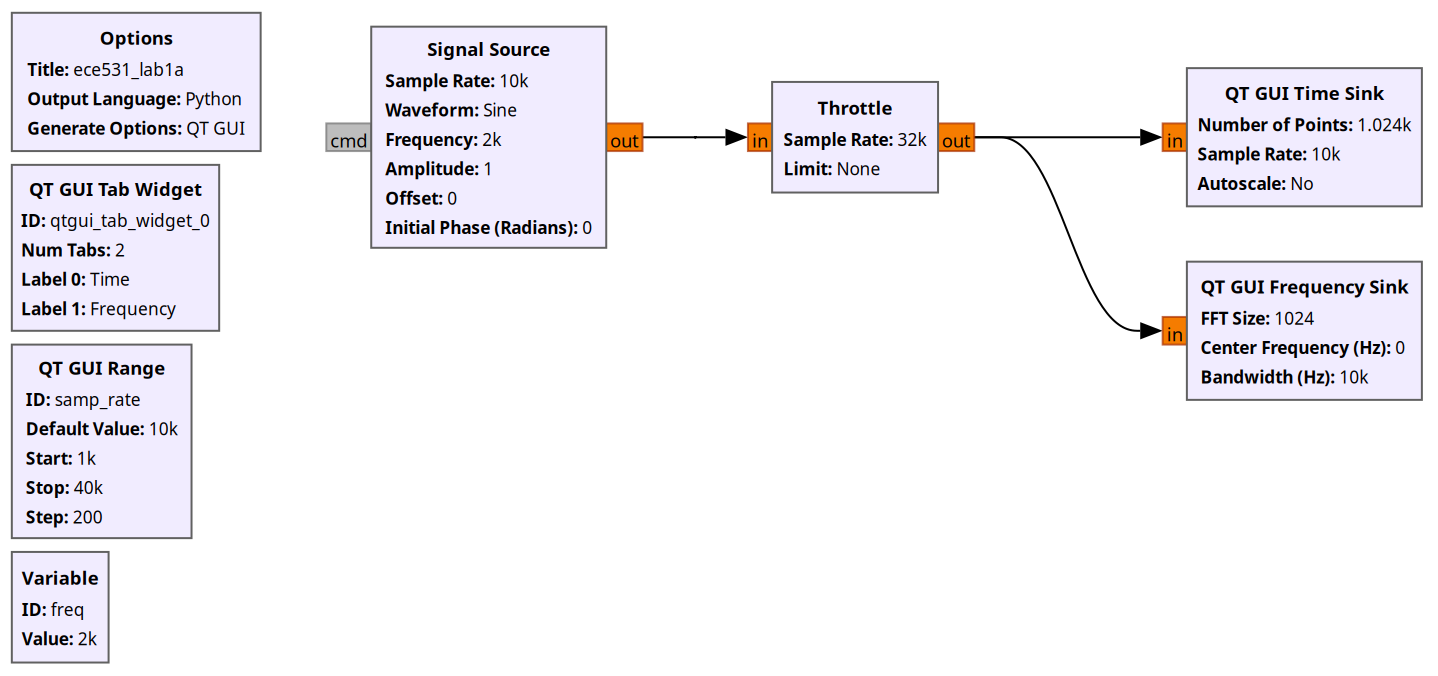
\includegraphics[width=0.7\textwidth]{sampling_rates_experiment.png}}}
	\caption{Setup for Sampling Rate Experiment}
	\label{fig::sampling_rates_experiment}
\end{figure}

We start by examining the signal when it is sampled at the 10 kHz default sample rate. We qualitatively analyze the time-domain signal by comparing it to an ideal sinusoid. We, then, measure the frequency of the signal. Next, we increase the sample rate to 40 kHz and compare the updated time and frequency plots to the previously collected data. Finally, we decrease the sample rate to 3.5 kHz and examine the frequency of the sampled signal.

\subsection{Complex Sampling \label{subsection::complex_sampling}}

In this section, we examine how complex sampling differs from real sampling. To perform our analysis, we modify the data types of the blocks in the GRC flowchart shown in Figure \ref{fig::sampling_rates_experiment}. The updated blocks use a "Complex Float 32" data type instead of a "Float 32" data type. Figure \ref{fig::complex_sampling_experiment} shows the updated block diagram. Note that the port colors have changed from orange to blue to reflect the change in data type.

\begin{figure}[H]
	\centerline{\fbox{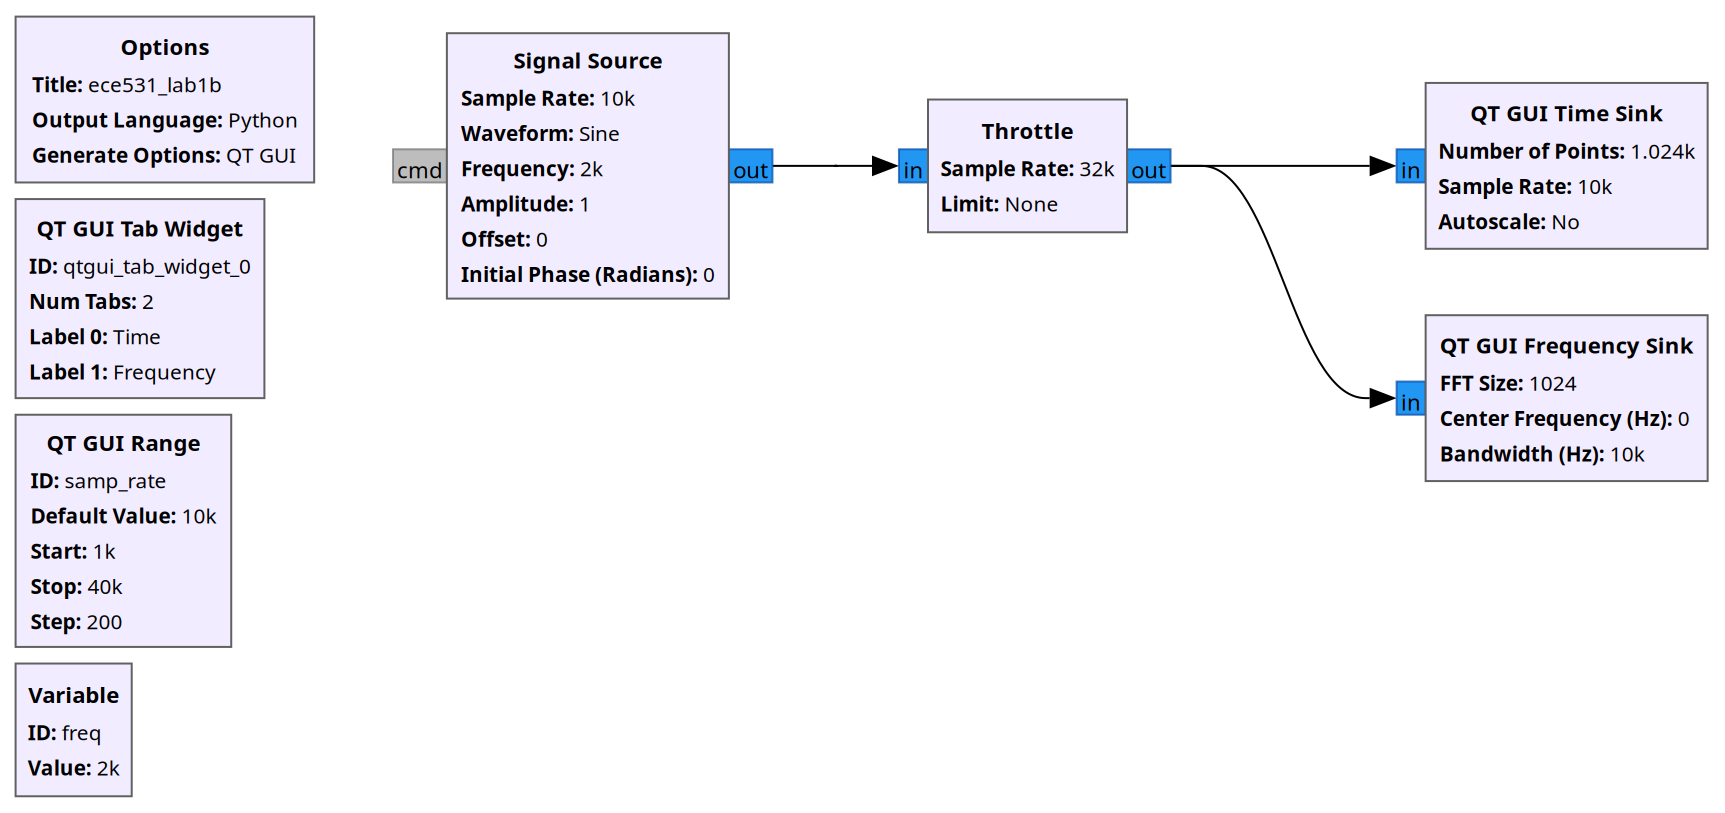
\includegraphics[width=0.7\textwidth]{complex_sampling_experiment.png}}}
	\caption{Setup for Complex Sampling Experiment}
	\label{fig::complex_sampling_experiment}
\end{figure}

Using the updated block diagram, we compare the updated frequency spectrum to the spectrum collected in subsection \ref{subsection::sampling_rates}, noting what happens to the positive and negative frequency components. We, then, investigate the time-domain signals and measure the phase between them. Next, we examine the signal amplitude on each channel while varying the sampling frequency from 10kHz to 40kHz. At the 40kHz sampling rate, we measure the frequency peak. Then, we measure the frequency peak at a 4kHz sampling rate. Finally, we continue decreasing the sampling rate and explain the location of the frequency peak.

\subsection{Frequency Observations}

In contrast to the previous sections, we now vary the frequency of the source while keeping the sampling rate constant. The experiment performed here reinforces the results of the previous sections and is performed on both real and complex-sampled data.
 
\subsubsection{Complex-sampled Flowgraph \label{subsection::frequency_observations_complex_sampling}}

The updated GRC flowchart for complex sampling is shown in Figure \ref{fig::frequency_observations_complex_sampling}. Compared with the previous flowchart, the sinusoid frequency can now be controlled with a slider.

\begin{figure}[H]
	\centerline{\fbox{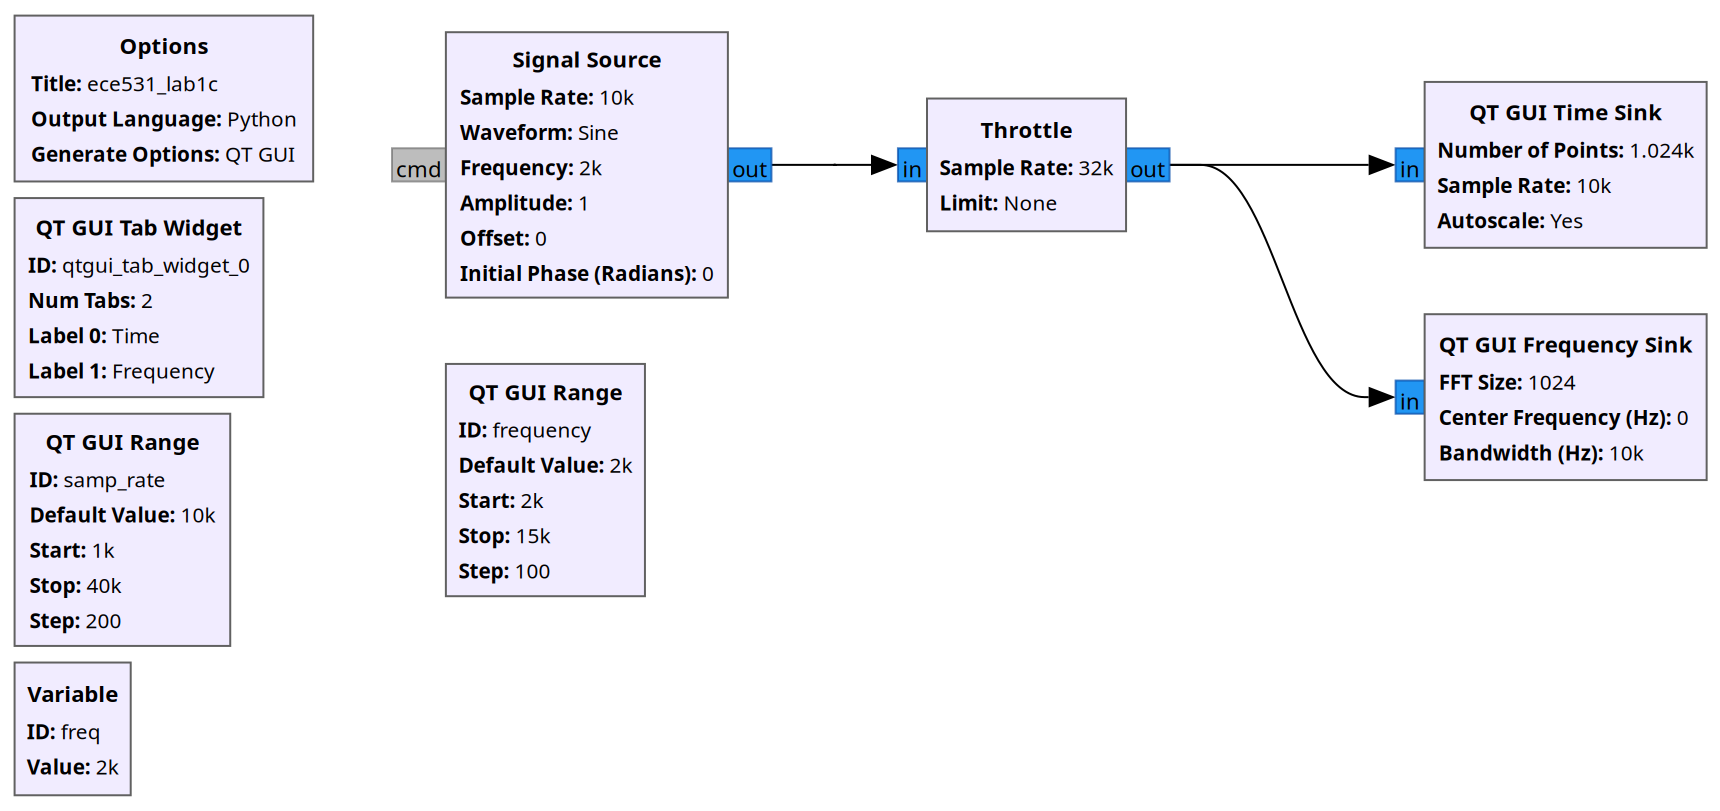
\includegraphics[width=0.7\textwidth]{frequency_observations_complex_sampling.png}}}
	\caption{Complex-sampled Frequency Observations}
	\label{fig::frequency_observations_complex_sampling}
\end{figure}

Using the updated flowchart, we vary the sinusoid frequency over its full range (from 2kHz to 15kHz), while observing the resulting spectrum. Based on the collected data, we notate any anomalies and describe why they occur. 

\subsubsection{Real-sampled Flowgraph}

We also investigate real-sampling using the flowchart shown in Figure \ref{fig::frequency_observations_real_sampling}. The flowchart is identical to the one shown in Figure \ref{fig::frequency_observations_complex_sampling} except for the data types which have been modified from "Complex Float 32" to "Float 32".

\begin{figure}[H]
	\centerline{\fbox{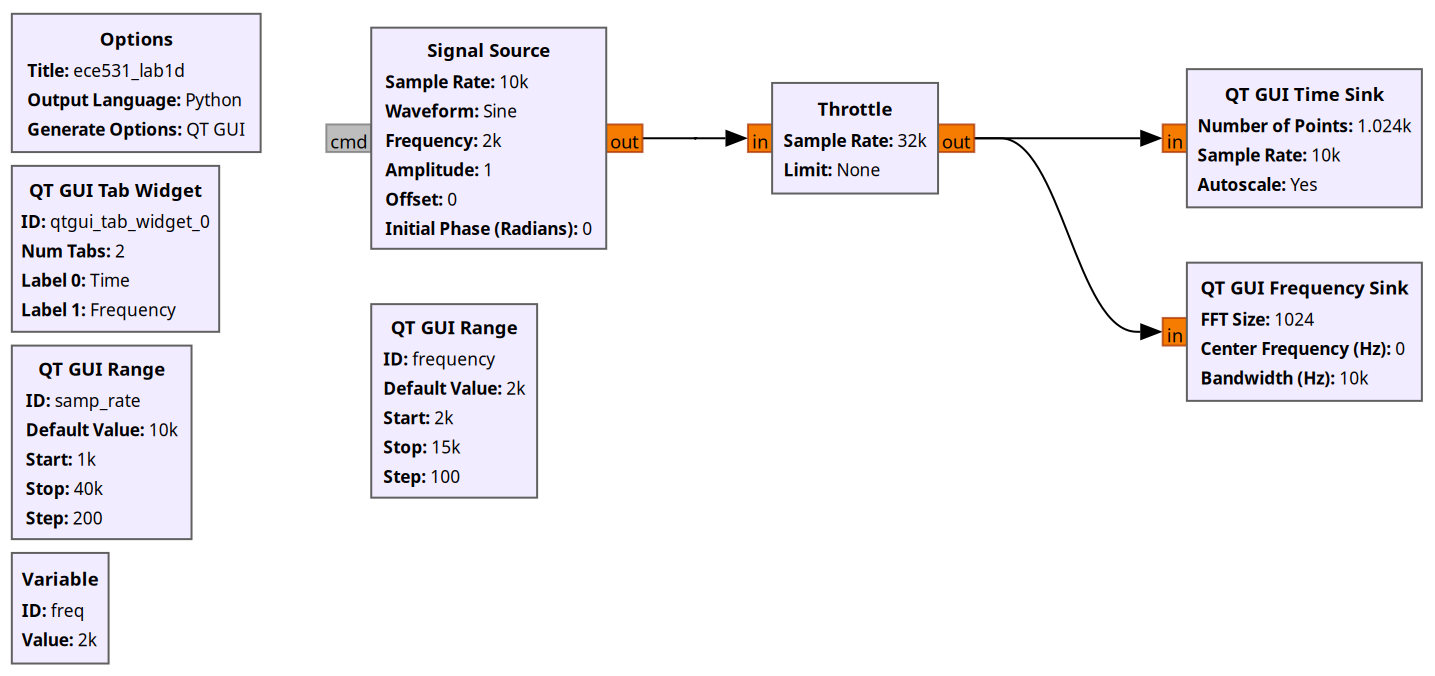
\includegraphics[width=0.7\textwidth]{frequency_observations_real_sampling.png}}}
	\caption{Real-sampled Frequency Observations}
	\label{fig::frequency_observations_real_sampling}
\end{figure}

Using the above flowchart, we vary the frequency of the sinusoid from its default value (10 kHz) to its maximum value (15 kHz). We observe the resulting spectrum and compare to the results we observed in Section \ref{subsection::frequency_observations_complex_sampling}.

\subsection{I/Q Imbalance}

In this section, we investigate the effect of I/Q imbalance on complex sampling. I/Q imbalance refers to a gain-phase mismatches in the I (in-phase) and Q (quadrature) paths. These gain-phase mismatches degrade the sampled signal and result in distortion. Figure \ref{fig::iq_imbalance_experiment} shows the GNU radio flowchart used to investigate I/Q imbalance.

\begin{figure}[H]
	\centerline{\fbox{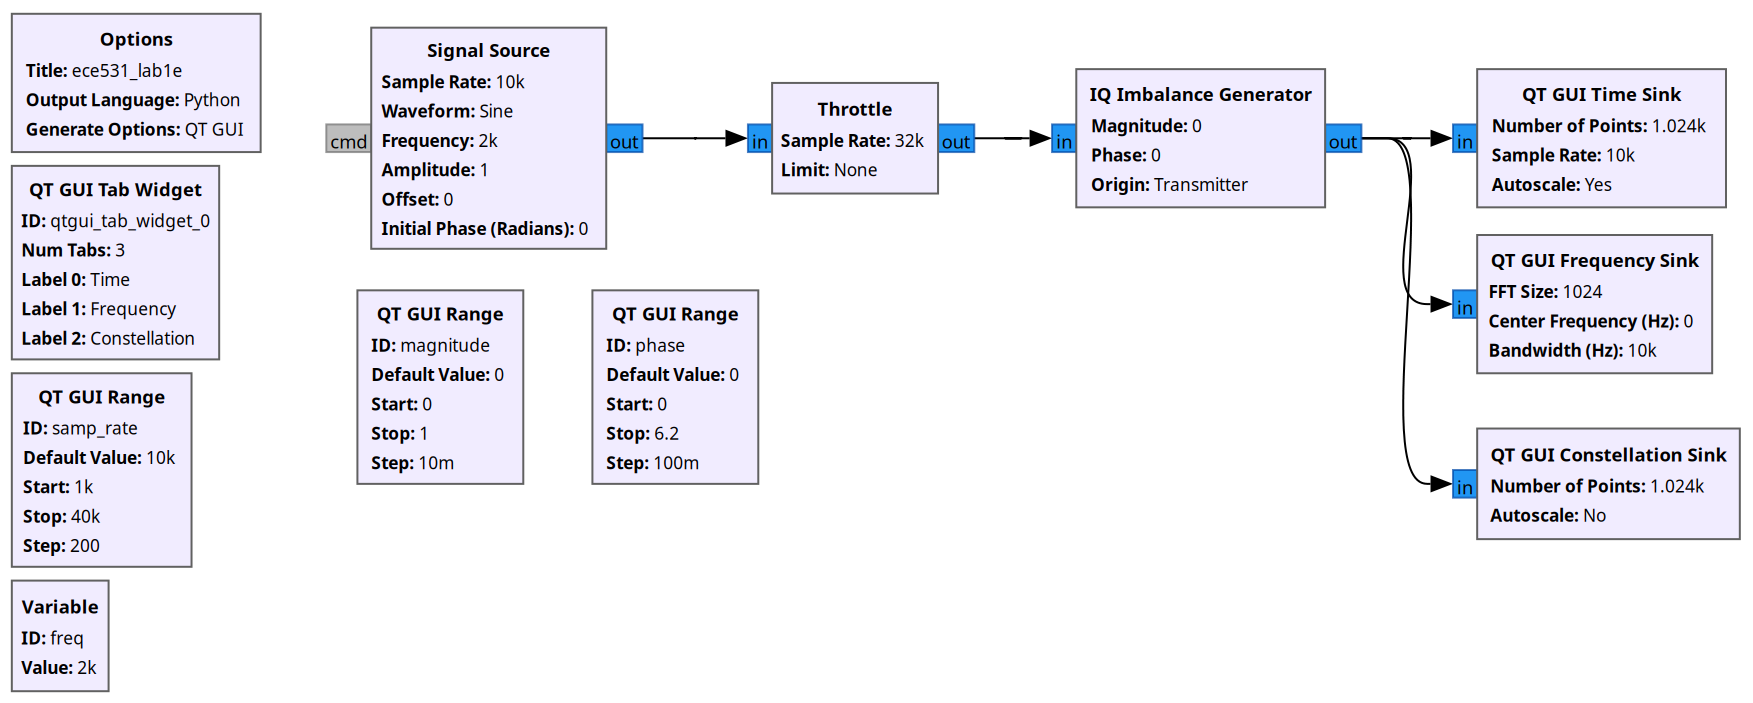
\includegraphics[width=0.7\textwidth]{iq_imbalance_experiment.png}}}
	\caption{I/Q Imbalance Experiment}
	\label{fig::iq_imbalance_experiment}
\end{figure}

\subsection{Adding Noise}

\subsection{Interpolation and Decimation}

\section{Results}
Results and discussion of the laboratory experiment, including captured outputs, observations, and responses to laboratory questions.

\section{Conclusion}
Conclusions to the overall lab that discuss meaningful lessons learned and other takeaways from the assignment. (Important)

%sampling rates
%complex samples
%interpolation
%decimation
%noise analysis

%\title{Lab 1 - Introduction to Software-Defined Radio\\
%
\includegraphics[scale=0.25\textwidth]{ua_logo.png}}
%\author{Owen Sowatzke}
%\date{\today}
%\maketitle

\end{document}